% !TEX TS-program = pdflatex
% !TEX encoding = UTF-8 Unicode

% This is a simple template for a LaTeX document using the "article" class.
% See "book", "report", "letter" for other types of document.

\documentclass[11pt]{article} % use larger type; default would be 10pt

\usepackage[utf8]{inputenc} % set input encoding (not needed with XeLaTeX)

%%% Examples of Article customizations
% These packages are optional, depending whether you want the features they provide.
% See the LaTeX Companion or other references for full information.

%%% PAGE DIMENSIONS
\usepackage{geometry} % to change the page dimensions
\geometry{a4paper} % or letterpaper (US) or a5paper or....
% \geometry{margin=2in} % for example, change the margins to 2 inches all round
% \geometry{landscape} % set up the page for landscape
%   read geometry.pdf for detailed page layout information

\usepackage{graphicx} % support the \includegraphics command and options

% \usepackage[parfill]{parskip} % Activate to begin paragraphs with an empty line rather than an indent

%%% PACKAGES
\usepackage{booktabs} % for much better looking tables
\usepackage{array} % for better arrays (eg matrices) in maths
\usepackage{paralist} % very flexible & customisable lists (eg. enumerate/itemize, etc.)
\usepackage{verbatim} % adds environment for commenting out blocks of text & for better verbatim
\usepackage{subfig} % make it possible to include more than one captioned figure/table in a single float
% These packages are all incorporated in the memoir class to one degree or another...

%%% HEADERS & FOOTERS
\usepackage{fancyhdr} % This should be set AFTER setting up the page geometry
\pagestyle{fancy} % options: empty , plain , fancy
\renewcommand{\headrulewidth}{0pt} % customise the layout...
\lhead{}\chead{}\rhead{}
\lfoot{}\cfoot{\thepage}\rfoot{}

%%% SECTION TITLE APPEARANCE
\usepackage{sectsty}
\allsectionsfont{\sffamily\mdseries\upshape} % (See the fntguide.pdf for font help)
% (This matches ConTeXt defaults)

%%% ToC (table of contents) APPEARANCE
\usepackage[nottoc,notlof,notlot]{tocbibind} % Put the bibliography in the ToC
\usepackage[titles,subfigure]{tocloft} % Alter the style of the Table of Contents
\renewcommand{\cftsecfont}{\rmfamily\mdseries\upshape}
\renewcommand{\cftsecpagefont}{\rmfamily\mdseries\upshape} % No bold!

%%% END Article customizations

%%% The "real" document content comes below...

\title{Modélisation distribuée d’un jeu stratégique : 
 \\ Cas d'une variante du jeu de dames}
\author{CHUPIN Pierre-Henri \\ SOLOMON Maria}
\date{} % Activate to display a given date or no date (if empty),
         % otherwise the current date is printed 

\begin{document}
\maketitle

\begin{abstract}
Ce  projet  a  pour  but  de  créer  une modélisation distribuée et de l'appliquer à un cas concré ici une variente du jeu de dames. Cela permettra de créer des stratégies pour des jeux et de comprendre mieux comment fonctionne la modélisation distribuée. \\
Mots-clés: Modélisation distribuée, stratégie, recherche de risque
\end{abstract}
\section{Introduction}
Ce projet s'inscrit dans le cadre du second semestre de Master 1 informatique de Lyon et dans l'optique de poursuivre en Master IA de Lyon. Pour ce projet nous avons put compter sur notre encadrant Aknine Samir appartenant à l'équipe Systèmes Multi-Agents de lyon. Depuis longtemps beaucoup d'informaticiens veulent résoudre des jeux comme les échecs en créant des IA cable de faire cela. Résoudre ce genre de problèmes demandes beaucoup de travail car il faut dans un premier temps créer informatiquement le jeux que l’on veut créer et mettre en place toutes ses règles. Une fois tout cela fait le vrai travail commence, le codage des stratégies que l’IA utilisera pour jouer au jeux. Nous avons décidé de faire la modélisation distribuée d'un jeu ancestrale, le jeu de dames. 

\section{Etat de l'art}

\subsection{Modélisation Distribuée}

\section{Outils utilisés}

\subsection{Le Jeu de dames}
La modélisation réalisé se base sur le jeux de dames classique mais avec quelque changement de régle qui permette d'avoir des comportements différents de ce qu'on peut voir en général. voici la liste des différentes régles et système utilisé utilisée:
\begin{itemize}
\item Un plateau carré de 10 cases sur 10
\item 20 pions blancs pour un joueur et 20 pions noir pour un autre joueur
\item chaque joueur jouera à tour de rôle et il pourra jouer 1 à N (nombre choisi avant de lancer une partie) pièces en même temps ce qui permet de voir comment vont réagir plusieurs pièces ensemble
\item Création classique de la dames qui permet d'avoir plusieurs types de pièce à gérer
\item Une dame peut se déplacer sur 3 cases de diagonale maximum nous avons voulu changer avec les règles habituels
\item La prise est obligatoire comme dans les règles classique des dames.
\item La prise multiple est possible aussi comme dans les dames classiques
\item Une partie est gagné si on prend toutes les pièces advairse ou si l'aderversaire ne peut pas ce déplacer quand c'est son tour de jeu.
\item Si il y a 30 coups sans prise la partie est nul
\end{itemize}

\section{Travail réalisé}

\subsection{Modélisation du jeu de dame}
Afin de commencé notre travail sur la modélisation distribuée nous avons du bien sur faire la modélisation du jeu de dame. Le fait de donner un aspect graphique au jeu ( on voit le plateau et les pièces ce déplacer) était important afin de mieux voir ce qu'il ce passe pendant le déroulement du programme et donner un coté graphique à notre travail. Bien sur on aurait pu le faire tourner sans affichage pour juste avoir le résultat de la simulation. Il a donc fallut partir à la recherche d'image pouvant être intégrer au projet qui permettrait de rendre cela possible. il nous fallait alors
\begin{itemize}
\item Une image de plateau carré de 10 cases sur 10
\item Une image de pion blanc et noir
\item Une image de dema blanche et noir
\end{itemize}
Une fois cela fait il nous suffit de mettre en place le plateau avec nos différentes images \cite{annexe1}. Voici donc à quoi ressemble le plateau et les pièces après le premier coup des blancs.

\begin{center}
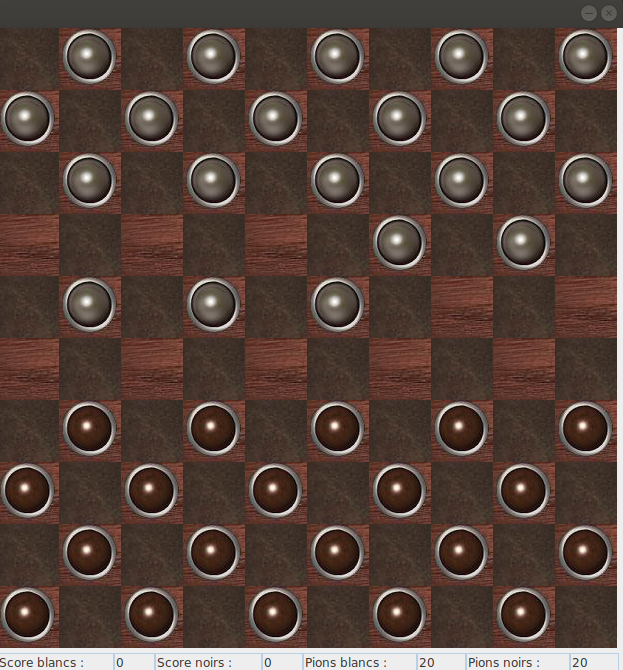
\includegraphics[scale=0.4]{plateau_ini}
\end{center}

afin de mieux pouvoir voir ce qu'il ce passe il a fallut mettre en place la possibilité de mettre en pause le jeu pour s'arreter et comprendre au mieux comment le programme fonctionne, nous verrons par la suite des exemples précis de comportement. \\

\subsection{Stratégie Naive}
Avant de pouvoir commencer à aller loin dans la modélisation distribuée nous avons du faire une stratégie naive qui consiste simplement à faire jouer l'IA le plus simplement possible sans aucune réflexion de sa part. Nous sommes partie sur le principe que l'IA jouera le maximum de pions possible pour chaque coups. Dans un premier temps elle regardera les coups obligatoires à faire comme la prise et jouera toute les prises, si il lui reste des mouvements possible elle devra alors regarder chaque pièce non déplacé si elle peut les déplacer. Si oui alors elle la joue qu'importe si le mouvement est mauvais ou non jusqu'à ne plus avoir de mouvement possible à jouer. cette stratégie naive nous servira de base pour créer une stratégie plus performante par la suite.

\subsection{Amélioration de la prise}



\section{Conclusion}


\end{document}
